This program models the flow around a 2D parabola at various Reynolds numbers ($Re$) and angles of attack ($\alpha$). A 2D parabola is a good model for the leading edge of a symmetric airfoil, such as the NACA 0012. This program is used to observe characteristics of the flow and to determine the angle of attack at which the flow seperates and stall occurs ($\alpha_{stall}(Re)$).

\begin{figure}[!ht]
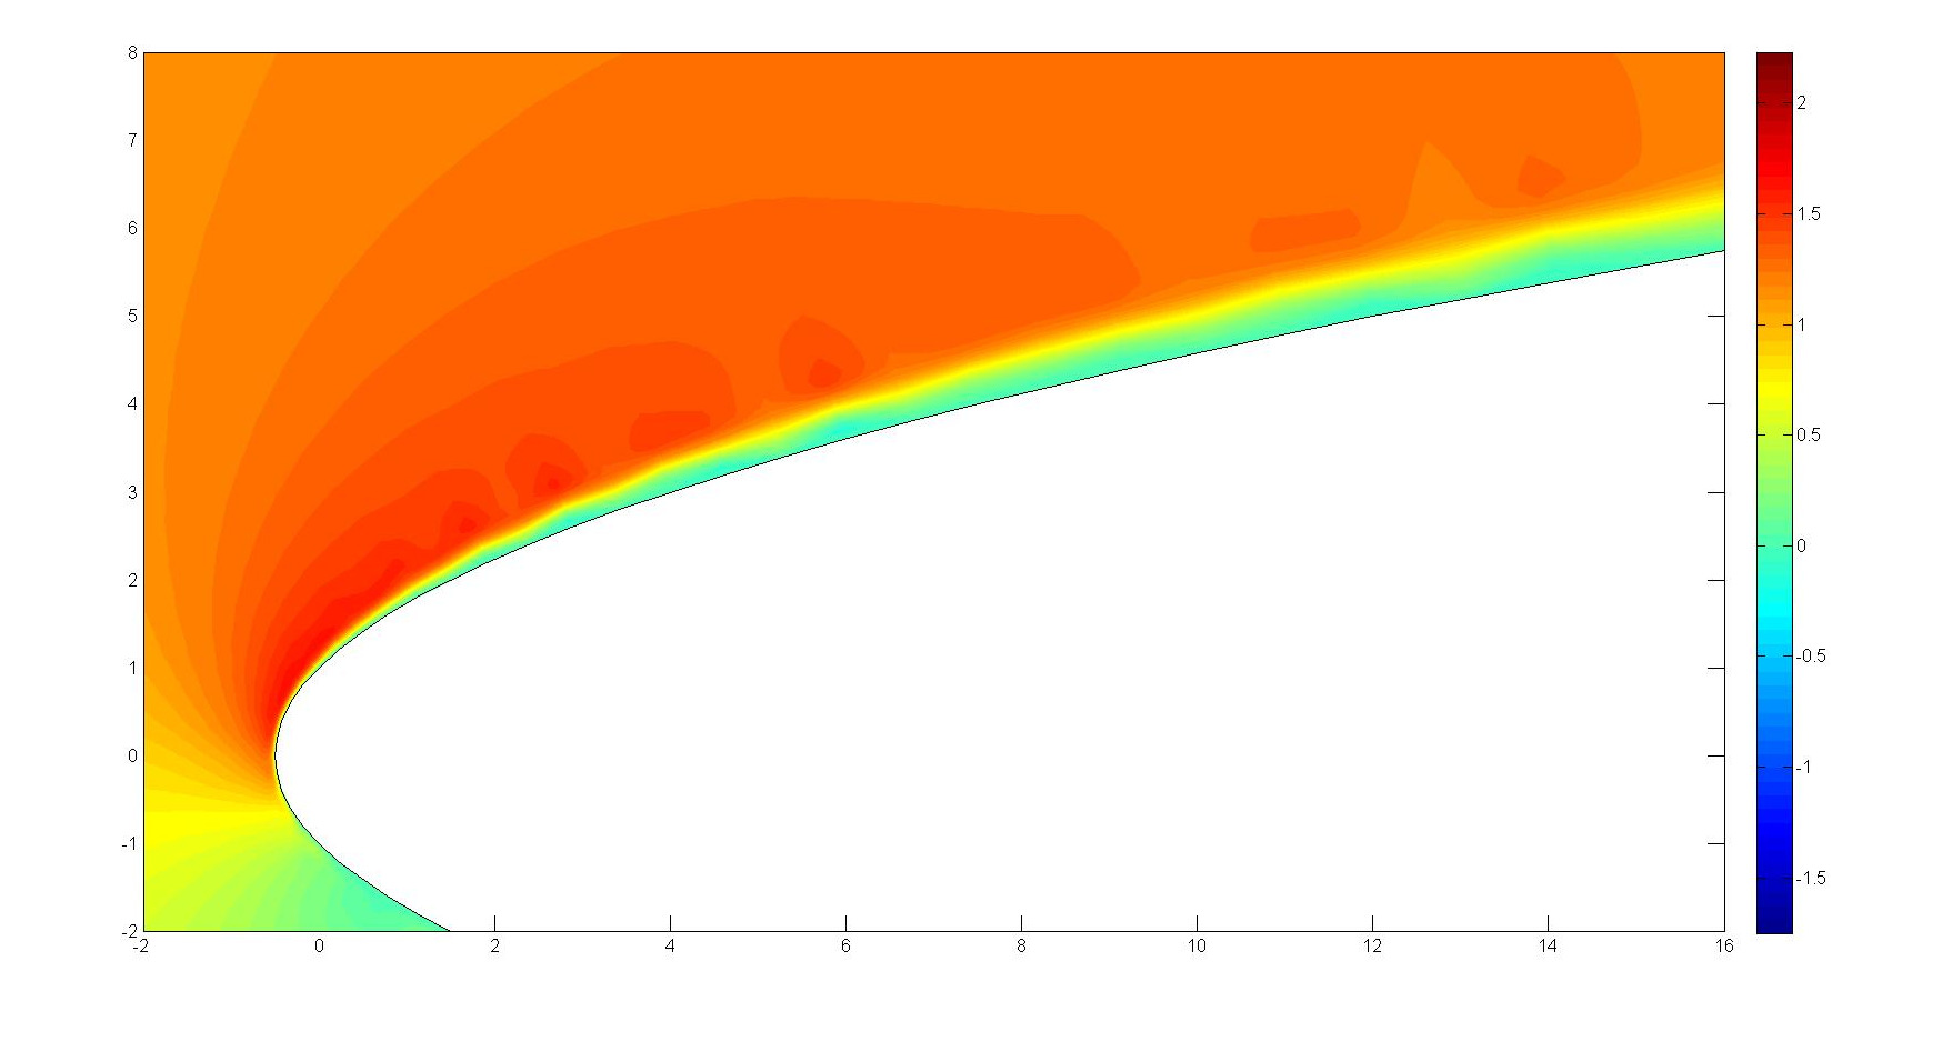
\includegraphics[width=\textwidth]{FF1p6.pdf}
\caption{Flow field for $Re_M = 700$, $\tilde{A} = 1.6$}
\label{fig:FF1p6}
\end{figure}

\begin{figure}[!ht]
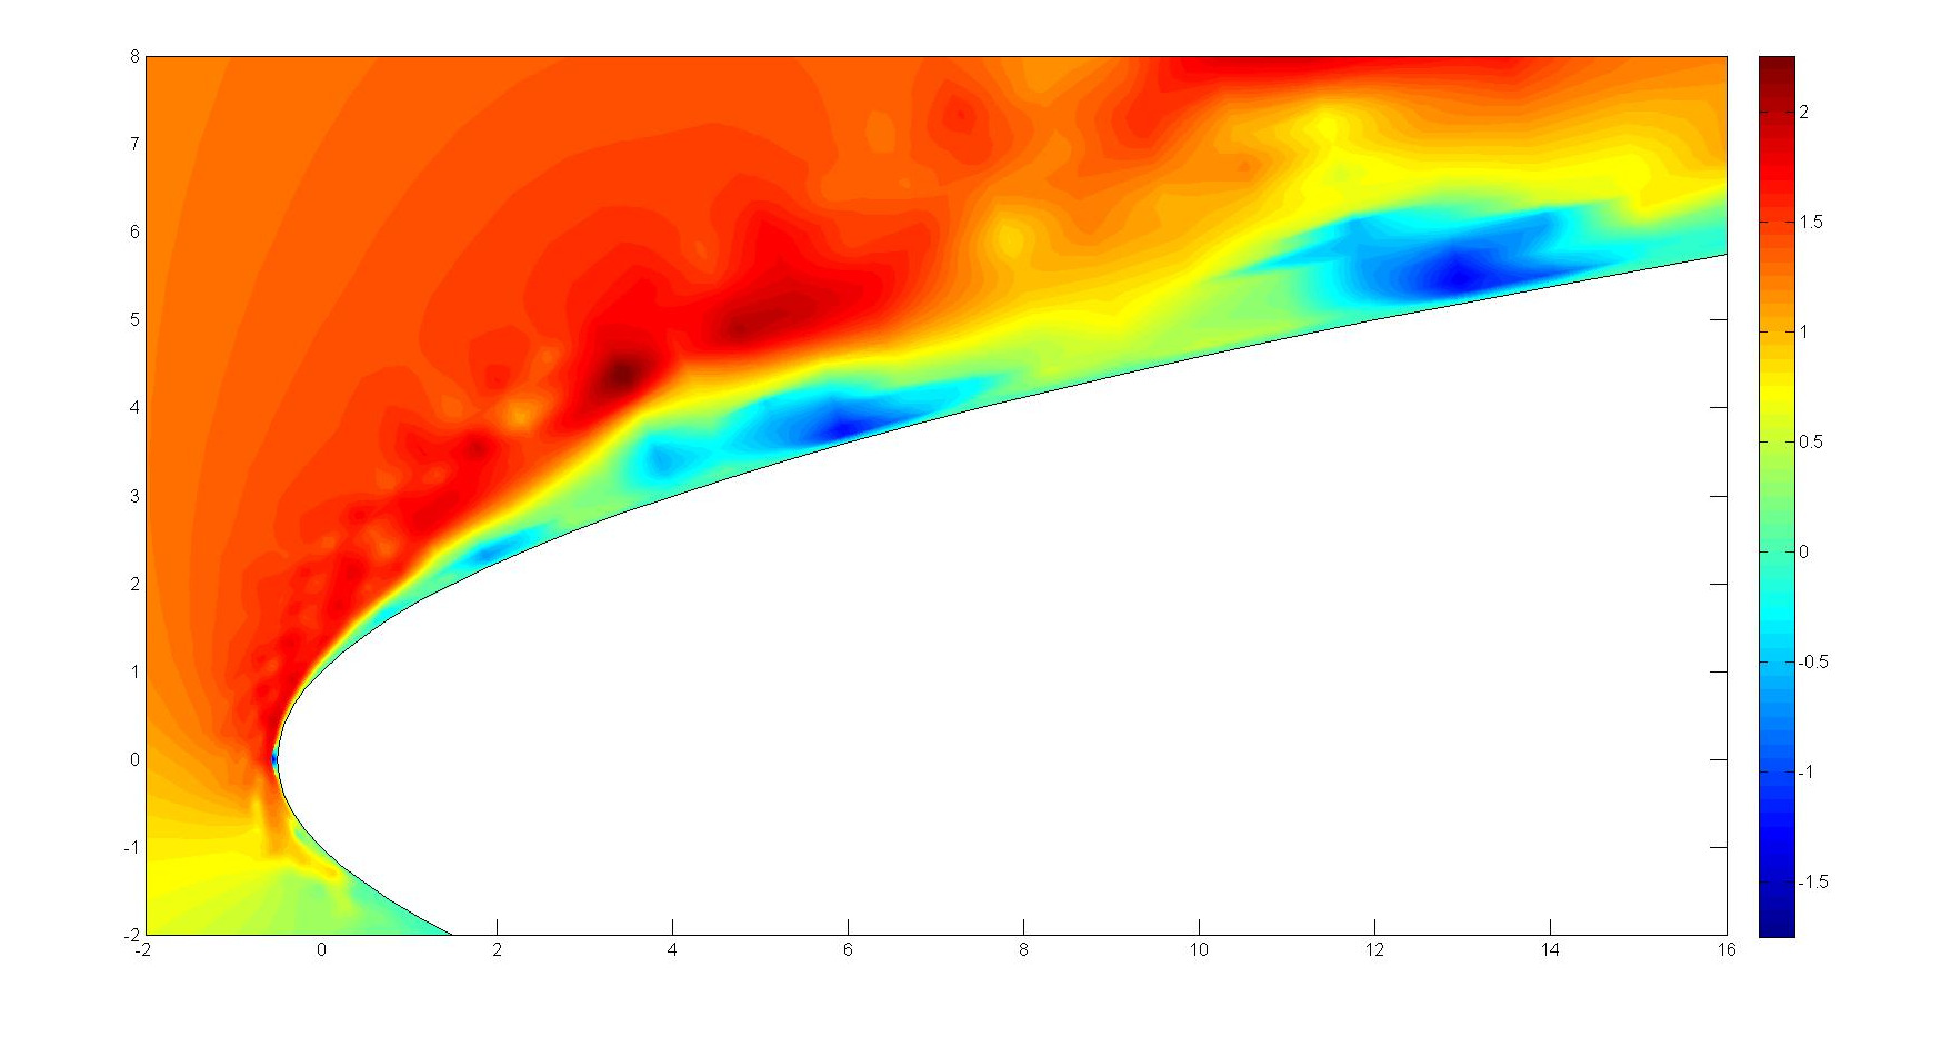
\includegraphics[width=\textwidth]{FF2p0.pdf}
\caption{$Re_M = 700$, $\tilde{A} = 2.0$}
\label{fig:FF2p0}
\end{figure}

To simulate the flow, the Navier-Stokes equations (\ref{eq:1}) are solved using an iterative method. In these equations, $x$ is the axial coordinate, $y$ is the perpendicular coordinate, , $u$ and $v$ are the axial and perpendicular velocities, respectivly, $p$ is the local pressure, and $Re_M$ is the Reynolds number $Re$ rescaled for computational purposes.

\[
\frac{\pd u}{\pd x} + \frac{\pd v}{\pd y} = 0
\]
\[
\frac{\pd u}{\pd t} + u \frac{\pd u}{\pd x} + v \frac{\pd u}{\pd y} = - \frac{\pd p}{\pd x} + \frac{1}{Re_M} \nabla^2 u
\]
\begin{equation}
\label{eq:1}
\frac{\pd v}{\pd t} + v \frac{\pd v}{\pd x} + v \frac{\pd v}{\pd y} = - \frac{\pd p}{\pd y} + \frac{1}{Re_M} \nabla^2 v
\end{equation}
%
Using
\begin{equation}
\label{eq:2}
u=\frac{\pd \psi}{\pd y},\: v=\frac{\pd \psi}{\pd x},\; \mathrm{and}\; \omega=\frac{\pd v}{\pd x} - \frac{\pd u}{\pd y},
\end{equation}
%
where $\psi$ is the stream function and $\omega$ is the vorticity, they can be reduced to:

\[
\frac{\pd \omega}{\pd t} + \frac{\pd \psi}{\pd y} \frac{\pd \omega}{\pd x} - \frac{\pd \psi}{\pd x} \frac{\pd \omega}{\pd y} = \frac{1}{Re_M} \nabla^2\omega
\]
\begin{equation}
\frac{\pd^2 \psi}{\pd x^2} + \frac{\pd^2 \psi}{\pd y^2} = -\omega.
\label{eq:4}
\end{equation}

Parabolic coordinates, $x=(\mu^2-\eta^2)/2$ and $y=\mu\eta$ are then used to transform the field into a Cartesian coordinate space. Here $\mu$ is the coordinate parallel to the surface of the parabola and $\eta$ is the coordinate normal to the surface. The parabolic surface is now described by the $\eta=1$ surface and flow evolves in the domain $-\infty < \mu < \infty$, $\eta> 1$. In parabolic coordinates the velocity components are given by:

\[
V_\mu=\frac{1}{\sqrt{\mu^2+\eta^2}} \frac{\pd \psi}{\pd \eta}, \quad\quad
V_\eta=\frac{-1}{\sqrt{\mu^2+\eta^2}} \frac{\pd \psi}{\pd \mu}
\]
% 
and (\ref{eq:4}) is given by
\[
\frac{\pd \omega}{\pd t} + \frac{1}{\mu^2 + \eta^2} \left[\frac{\pd}{\pd \mu} \left(\sqrt{\mu^2 + \eta^2} V_\eta \omega \right) \right] = \frac{1}{Re_M(\mu^2 + \eta^2)} \left(\frac{\pd^2 \omega}{\pd \mu^2} + \frac{\pd^2 \omega}{\pd \eta^2} \right)
\]

\begin{equation}
\label{eq:7}
\omega = \frac{-1}{\mu^2 + \eta^2} \left(\frac{\pd^2 \psi}{\pd \mu^2} + \frac{\pd^2 \psi}{\pd \eta^2} \right)
\end{equation}

Equation \ref{eq:7} is subjected to the tangency and no slip boundary conditions on the parabola surface, i.e. $V_\eta(\mu,\eta=1) = 0$, $\psi(\mu,\eta=1) = 0$, as well as boundary conditions on the far field.

For a numerical implementation, the semi-infinite domain $\eta > 1$ is reduced to the domain $-\mu_{max} < \mu < \mu_{max}$ and $1 < \eta < \eta_{max}$, where $\mu_{max}$ and $\eta_{max}$ are sufficiently large. This domain is discretized by a uniform mesh with constant step sizes in both directions $\Delta \mu$ and $\Delta \eta$ espectively. The index of each grid point is ($i$,$j$) respectively, where $-M \le i \le M$, $1 \le j \le N$. Time is discretized by constant time steps $\Delta t$ with index $n$ for each time level. The time
derivative in (\ref{eq:7}) is approximated by a first-order forward difference and second-order central
differences are used to approximate the spatial derivatives. The discretized formulation of (\ref{eq:7}) is:

\[
\frac{\omega^{n+1}_{i,j}+\omega^n_{i,j}}{\Delta t} + \frac{1}{s^2_{i,j}}
\]
\[
\cdot \left(
\frac{s_{i+1,j}V^n_{\mu_{i+1,j}}\omega^n_{i+1,j}-s_{i-1,j}V^n_{\mu_{i-1,j}}\omega^n_{i-1,j}}
     {2\Delta\mu}
+
\frac{s_{i,j+1}V^n_{\mu_{i,j+1}}\omega^n_{i,j+1}-s_{i,j-1}V^n_{\mu_{i,j-1}}\omega^n_{i,j-1}}
     {2\Delta\eta}
\right)
\]
\begin{equation}
\label{eq:9}
=\frac{1}{Re_M s^2_{i,j}}
\left(
\frac{\omega^n_{i-1,j}-2\omega^n_{i,j}+\omega^n_{i+1,j}}{(\Delta\mu)^2}
+
\frac{\omega^n_{i,j-1}-2\omega^n_{i,j}+\omega^n_{i,j-1}}{(\Delta\eta)^2}
\right)
\end{equation}
where $s_{i,j}=\sqrt{\mu^2_{i,j}+\eta^2_{i,j}}$.
Equation \ref{eq:9} is rearranged to solve for $\omega^{n+1}_{i,j}$ in terms of the fields of
vorticity and velocity at time level $n$.
Once the vorticity field is progressed in time, the stream
function at time level $n+1$ is solved using spatial central differences:
\begin{equation}
\label{eq:10}
\frac{\psi^{n+1}_{i-1,j}-2\psi^{n+1}_{i,j}+\psi^{n+1}_{i+1,j}}{(\Delta\mu)^2}+
\frac{\psi^{n+1}_{i,j-1}-2\psi^{n+1}_{i,j}+\psi^{n+1}_{i,j+1}}{(\Delta\eta)^2}
=-\omega^{n+1}_{i,j}
\end{equation}

Equation \ref{eq:10} is solved by the Jacobi iteration method. Once convergence to a given tolerance is achieved, the velocity field at time level $n+1$ can be determined from:

\[
V_\mu^{n+1}=\frac{1}{\sqrt{\mu_{i,j}^2+\eta_{i,j}^2}} \frac{\psi_{i,j+1}^{n+1} - \psi_{i,j-1}^{n+1}}{2\Delta \eta},
\]
\begin{equation}
\label{eq:11}
V_\eta^{n+1}=\frac{-1}{\sqrt{\mu_{i,j}^2+\eta_{i,j}^2}} \frac{\psi_{i+1,j}^{n+1} - \psi_{i-1,j}^{n+1}}{2\Delta \mu}
\end{equation}

The field of velocity and vorticity at time level $n+1$ are used to advance the solution to the next time step. For a given $Re_M$ and $\tilde{A}$, where $\tilde{A}$ is a variable related to $\alpha$, the solution of (\ref{eq:9}) through (\ref{eq:11}) is advanced in time until time-asymptotic behavior, steady or periodic, is achieved.

The computations are initiated in the following way. At a given $Re_M$ and $\tilde{A} = 0$, the inviscid, potential flow solution is used as the initial state and a simulation is run until a steady, time-asymptotic state of the viscous flow problem is found. This solution is then used as an initial state for the computation of the flow at the same $Re_M$  and an increased value of $\tilde{A}$ , for example $\tilde{A} = 0.1$. This process is repeated for increasing $\tilde{A}$.

An additional aspect of this program is it's ability to simulate synthetic jets on the parabolic surface. A synthetic jet is a small oscillating surface which introduces pulses of air into the flow at a particular frequency. There are experimental results which show that flow seperation can be reduced, lift increased, and the onset of stall delayed if these jets are properly placed and oscillated at a specific frequency. This location and frequency is dependent on the characteristics of the flow including the Reynolds number and the corresponding shedding frequency at a particular angle of attack. By modifying jet location and frequency and observing the effect on the simulation, this program allows the ideal values for these parameters to be determined.

\begin{figure}[!ht]
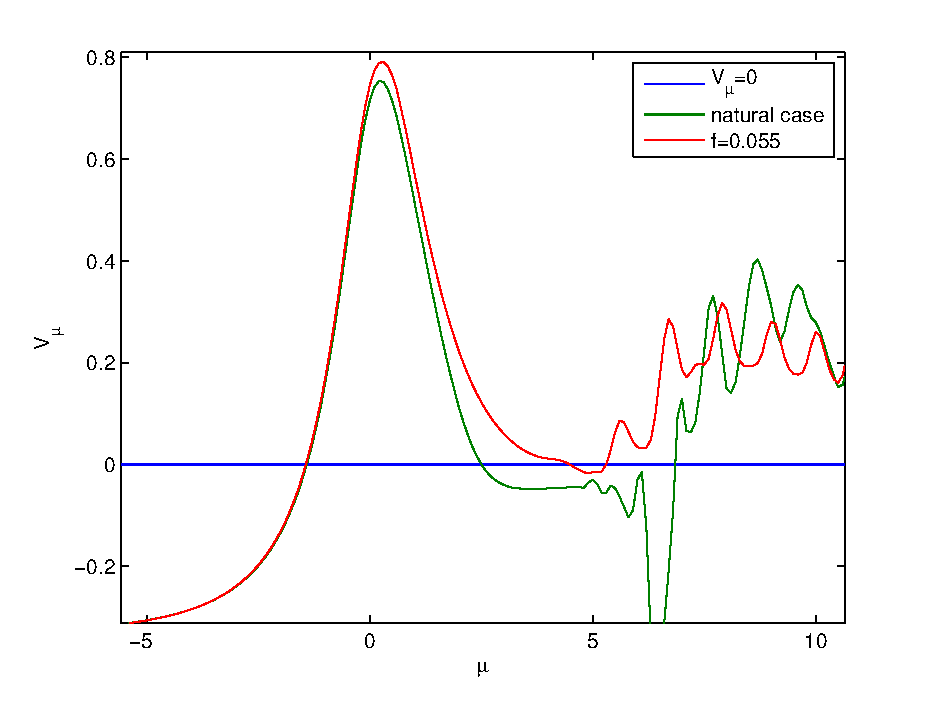
\includegraphics[width=\textwidth]{jets.pdf}
\caption{Effect of jet on $\mu$ velocity}
\label{fig:jets}
\end{figure}


The effect of this can be seen in Figure \ref{fig:jets}. By adding a synthetic jet near the stagnation point, the peak velocity was increased and the seperation bubble (negitive portion after the peak) was reduced in size. The effect of this is increased lift and reduced drag, which in practical use translates to better fuel efficiency.



\end{document}

